

\tikzset{every picture/.style={line width=0.75pt}} %set default line width to 0.75pt        

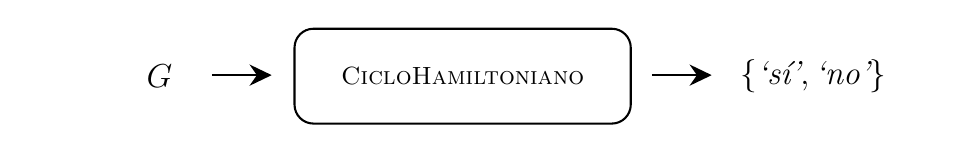
\begin{tikzpicture}[x=0.75pt,y=0.75pt,yscale=-1,xscale=1]
%uncomment if require: \path (0,629); %set diagram left start at 0, and has height of 629

%Rounded Rect [id:dp014958459164192917] 
\draw   (250,537.64) .. controls (250,532.59) and (254.09,528.5) .. (259.14,528.5) -- (402.86,528.5) .. controls (407.91,528.5) and (412,532.59) .. (412,537.64) -- (412,565.06) .. controls (412,570.11) and (407.91,574.2) .. (402.86,574.2) -- (259.14,574.2) .. controls (254.09,574.2) and (250,570.11) .. (250,565.06) -- cycle ;
%Straight Lines [id:da560650477859397] 
\draw    (210.17,550.86) -- (236,550.86) ;
\draw [shift={(239,550.86)}, rotate = 180] [fill={rgb, 255:red, 0; green, 0; blue, 0 }  ][line width=0.08]  [draw opacity=0] (10.72,-5.15) -- (0,0) -- (10.72,5.15) -- (7.12,0) -- cycle    ;
%Straight Lines [id:da283131752424681] 
\draw    (422.17,550.86) -- (448,550.86) ;
\draw [shift={(451,550.86)}, rotate = 180] [fill={rgb, 255:red, 0; green, 0; blue, 0 }  ][line width=0.08]  [draw opacity=0] (10.72,-5.15) -- (0,0) -- (10.72,5.15) -- (7.12,0) -- cycle    ;

% Text Node
\draw (331,551.35) node  [font=\small] [align=left] {\begin{minipage}[lt]{109.82pt}\setlength\topsep{0pt}
\begin{center}
\textsc{CicloHamiltoniano}
\end{center}

\end{minipage}};
% Text Node
\draw (184.98,551.35) node  [font=\large] [align=left] {\begin{minipage}[lt]{88.65pt}\setlength\topsep{0pt}
\begin{center}
$G$
\end{center}

\end{minipage}};
% Text Node
\draw (500,551.35) node  [font=\large] [align=left] {\begin{minipage}[lt]{88.4pt}\setlength\topsep{0pt}
\begin{center}
$\{\text{\emph{`sí'}}, \text{\emph{`no'}}\}$
\end{center}

\end{minipage}};


\end{tikzpicture}
